\documentclass[11pt]{article}
\usepackage[a4paper,margin=1in]{geometry}
\usepackage{graphicx}
\usepackage{booktabs}
\usepackage{amsmath}
\usepackage{hyperref}

\title{Self-Supervised Pretraining for Low-Shot Motor-Imagery EEG Calibration}
\author{Anonymous for review}
\date{}

\begin{document}
\maketitle

\begin{abstract}
Motor-imagery (MI) brain-computer interfaces require per-user calibration data. We evaluate whether compact self-supervised learning (SSL) reduces the labeled trials needed for calibration. We benchmark CSP+LDA, EEGNet from scratch, masked SSL, and physiology-inspired $\mu/\beta$ SSL under identical few-shot protocols across multiple MI datasets.
\end{abstract}

\section{Introduction}
\subsection{Calibration bottleneck in MI-BCI}
MI decoders often require tens of labeled trials per class, limiting usability in clinical and home settings.
\subsection{Related work}
Summarize CSP/FBCSP, deep MI decoding, and SSL for EEG representation learning.
\subsection{Gap and contributions}
\begin{itemize}
\item Reproducible few-shot calibration benchmark with fixed split protocol.
\item Compact (\(<100\)k params) SSL encoder and transfer settings.
\item Multi-dataset and cross-dataset evidence with statistical testing and deployment metrics.
\end{itemize}

\section{Methods}
\subsection{Datasets and splits}
BNCI2014-001, BNCI2014-004 (or Cho2017), PhysionetMI (subjects 1--20). Few-shot budgets: 5/10/20/50 trials per class, 5 repeats.
\subsection{Models}
CSP+LDA, EEGNet from scratch, masked SSL encoder, $\mu/\beta$ SSL encoder.
\subsection{Pretraining objectives}
Masked reconstruction and $\mu/\beta$ contrastive pretext.
\subsection{Few-shot evaluation modes}
Frozen linear probe and full fine-tuning.
\subsection{Statistics}
Paired t-tests, Bonferroni correction, Cohen's $d$, and power analysis.

\section{Results}
\subsection{Main few-shot calibration curves}
Insert Figure~\ref{fig:main_curves}.
\begin{figure}[h]
\centering
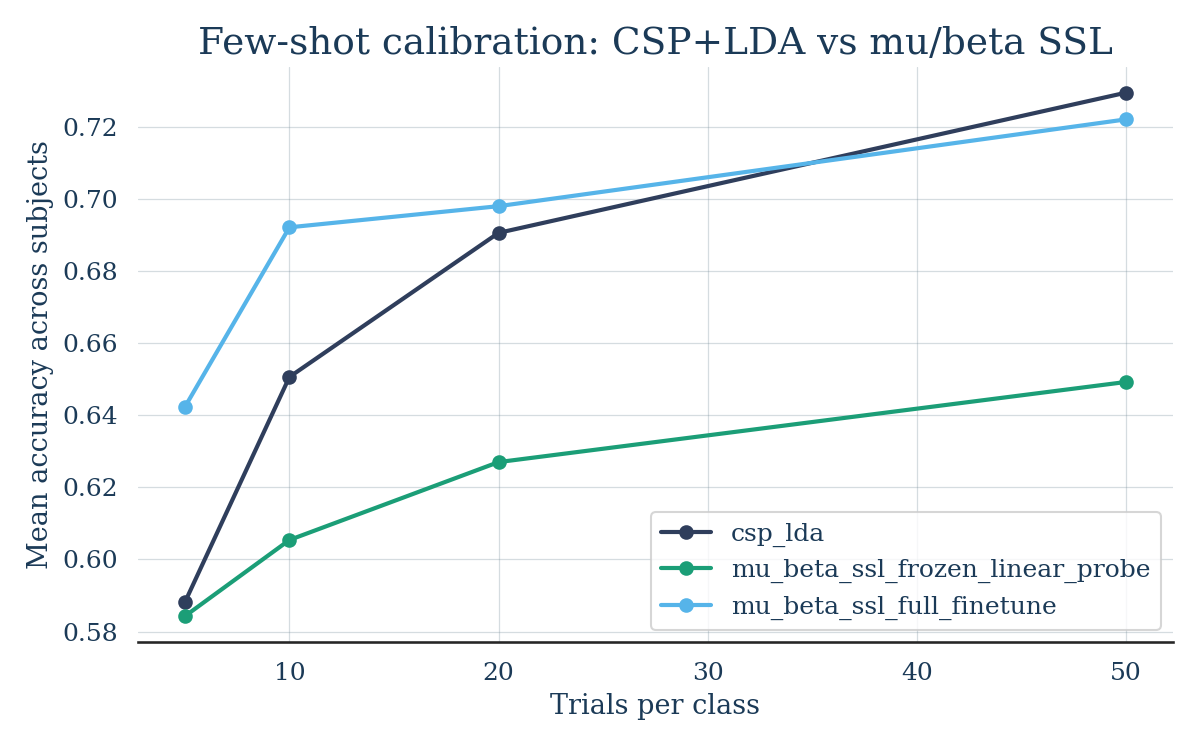
\includegraphics[width=0.8\textwidth]{results_mu_beta_ssl_vs_csp.png}
\caption{Few-shot calibration comparison on BNCI2014-001.}
\label{fig:main_curves}
\end{figure}

\subsection{Three-dataset summary table}
Insert Table with CSP, EEGNet, masked SSL and $\mu/\beta$ SSL.

\subsection{Cross-dataset transfer}
Pretrain on BNCI and evaluate few-shot transfer on PhysionetMI.

\subsection{Failure diagnosis}
Include embedding visualization and projection-head ablation (Figure~\ref{fig:failure}).
\begin{figure}[h]
\centering
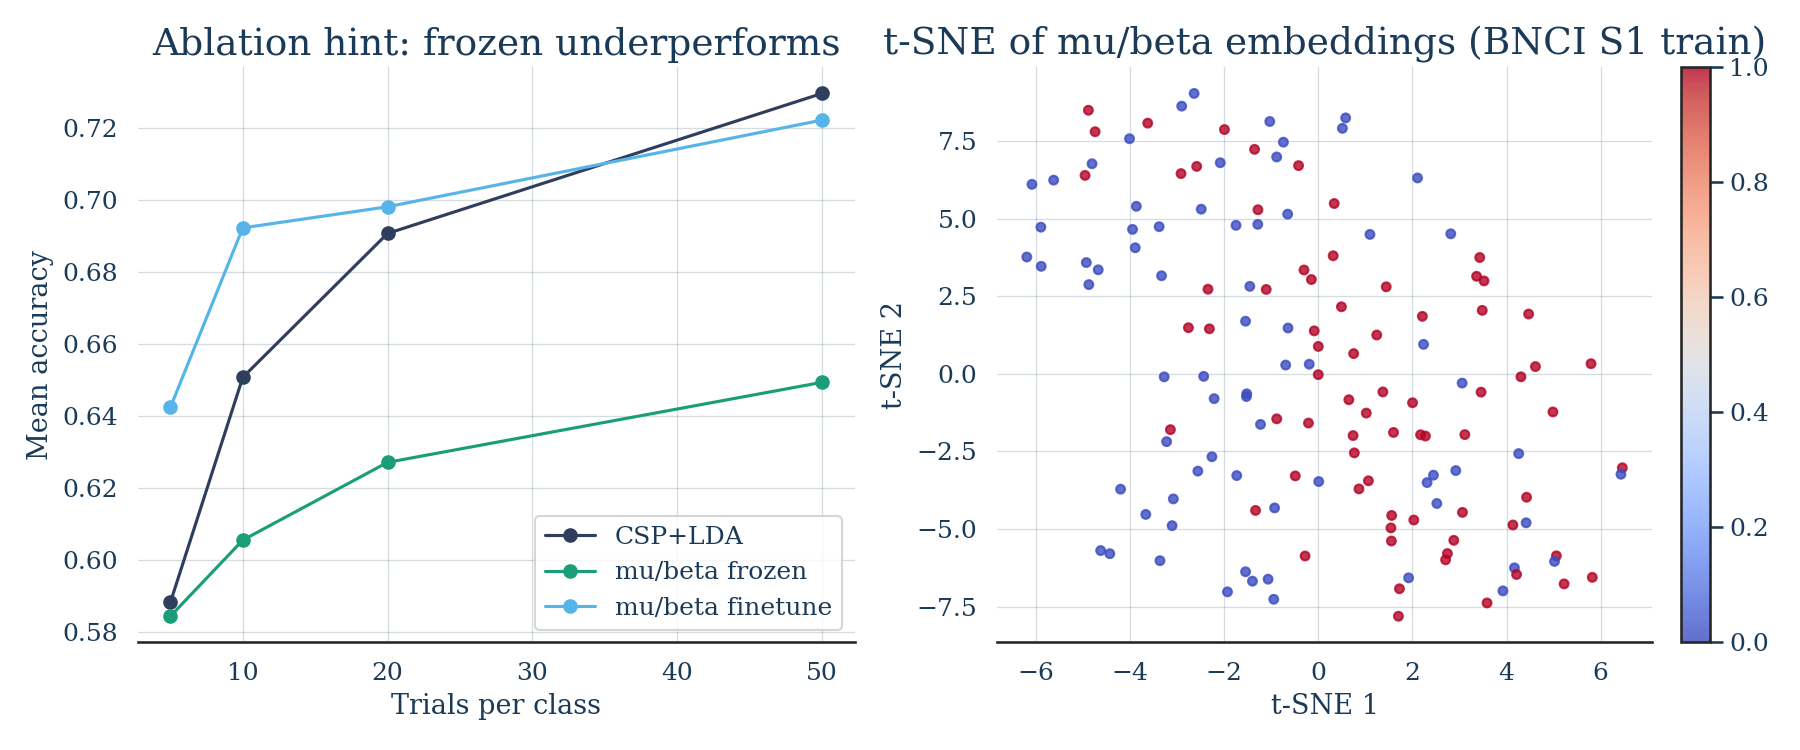
\includegraphics[width=0.9\textwidth]{mu_beta_failure_analysis.png}
\caption{Failure diagnosis: embedding structure and ablation trends.}
\label{fig:failure}
\end{figure}

\subsection{Deployment metrics}
Report ONNX latency, VRAM footprint, and int8 quantization drop.

\section{Discussion}
\subsection{Why generic SSL may outperform physiology priors in low-data}
Discuss representational flexibility versus hand-crafted priors.
\subsection{Limitations}
Dataset scope, inter-subject variance, and computational constraints.
\subsection{Clinical implications}
Potential reduction in calibration burden for MI-BCI deployment.

\section{Reproducibility checklist}
Code/scripts, seeds, versions, and data-access instructions.

\section{Conclusion}
Compact SSL can reduce MI calibration requirements under a strict few-shot protocol.

\bibliographystyle{plain}
\bibliography{references}

\end{document}
